\chapter{序論}

\section{研究背景}
  \subsection{宇宙天気}
  宇宙天気とは、太陽活動に起因する宇宙環境の現象を指し、激しい宇宙天気の変動は地球の磁場や電離層、大気圏に影響を与える(図\ref{fig:space_weather_impact})。
  これは大規模なものであれば、地球上の電力網や衛星通信など、人間の技術システムに壊滅的被害をもたらす可能性がある。
  そのため、宇宙天気を予測することは、人間の技術システムを宇宙天気の影響から守るための重要な課題である。
  \begin{figure}[htbp]
    \centering
    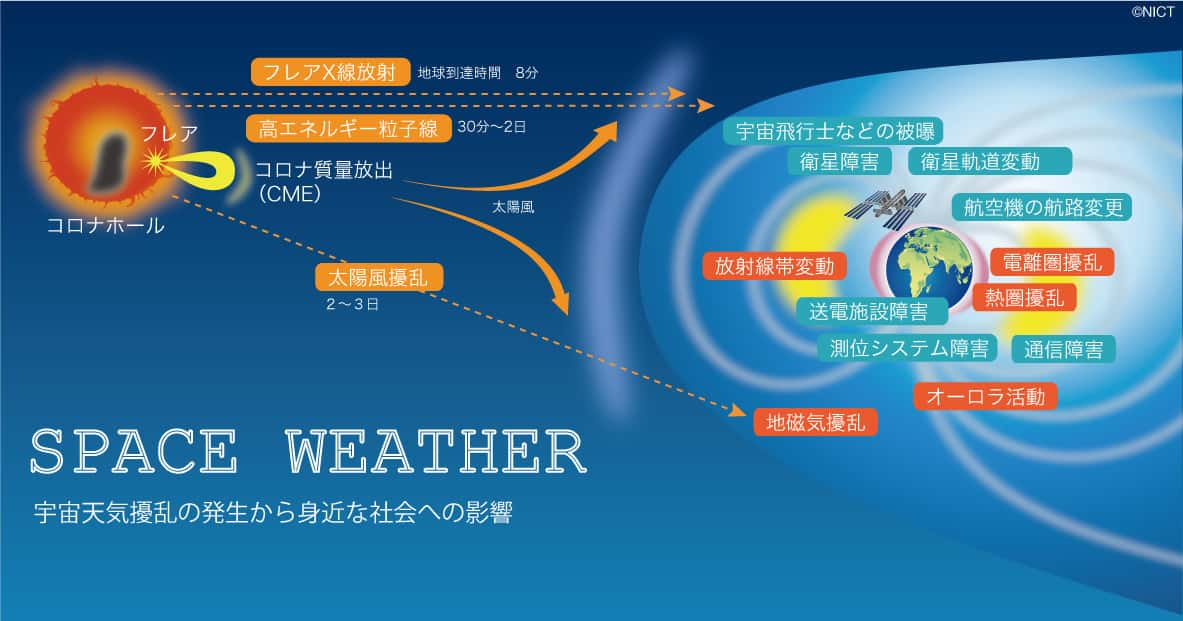
\includegraphics[width=0.9\textwidth]{figures/spaceweather.jpg}
    \caption[宇宙天気擾乱と社会への影響]{宇宙天気擾乱の発生と社会への影響の概念図。出典: 国立情報通信研究所, 「宇宙天気予報とは」, \url{https://swc.nict.go.jp/knowledge/relation.html}(アクセス日: 2024年1月9日)}
    \label{fig:space_weather_impact}
  \end{figure}

  太陽の表面や大気における物理現象、特に太陽フレアやコロナ質量放出(CME)などの爆発的なイベントは、地球に到達する高エネルギー粒子や放射線の量を増加させ、宇宙天気に大きな影響を与える。
  宇宙天気を予報するためには、そういった太陽イベントを観測し、それらの観測データを解析することが必要である。
  実際の宇宙天気予報は、これらの観測データを入力としたシミュレーションモデルや機械学習モデルを常に実行し、さらに定期的に専門家による主観的な予報を行うことが多い。

  % 宇宙天天気予報のための観測
  % 観測の重要性
  % 観測をもとにモデルを実行したり主観的な分析をして数日先の予報を行う
  \subsection{観測データ}
  刻一刻と変化する太陽の状態から宇宙天気を予報するために、高精度な観測データは必要不可欠である。
  観測は、さまざまな観測機器を搭載した観測衛星に加え、世界各国に存在する地上の望遠鏡や電波望遠鏡などで行われる。
  Solar Dynamics Observatory (SDO) (\citex{pesnell2012solar})や、Solar and Heliospheric Observatory (SOHO) (\citex{domingo1995soho})、「ひので」 (\citex{kosugi2008hinode})などの太陽観測衛星からリアルタイムで提供される、太陽の表面や大気の観測データは非常に重要である。

  後述するDeep Flare Netなどに代表される太陽フレア予測モデルでは、SDOに搭載されたHelioseismic and Magnetic Imager (HMI) (\citex{scherrer2012helioseismic})や、Atmospheric Imaging Assembly (AIA) (\citex{lemen2012atmospheric})から得られる磁場データや紫外線データ(図\ref{fig:sdo_axmple})を入力として、数時間後から数日後までの太陽フレアの発生を予測する。
  Magnetohydrodynamics (MHD)シミュレーションモデルに代表される多くの数値シミュレーションモデルにおいても、それらの衛星から得られた太陽表面のデータを入力として予測を行う。
  例えば、\citex{shiota2016magnetohydrodynamic}, \citex{shiota2021susanoo}による太陽嵐予測システムSUSANOO-CMEは、実際に運用されている高性能なシミュレーションモデルであり、SOHOやSDOなどの複数の太陽観測衛星による得られたコロナグラフや極紫外線データを入力とする。
  これをもとに太陽風、CMEの伝搬をシミュレーションすることで、いち早く太陽嵐の到達時刻を予測することができる。
  \begin{figure}[htbp]
    \begin{subfigure}{0.5\textwidth}
      \centering
      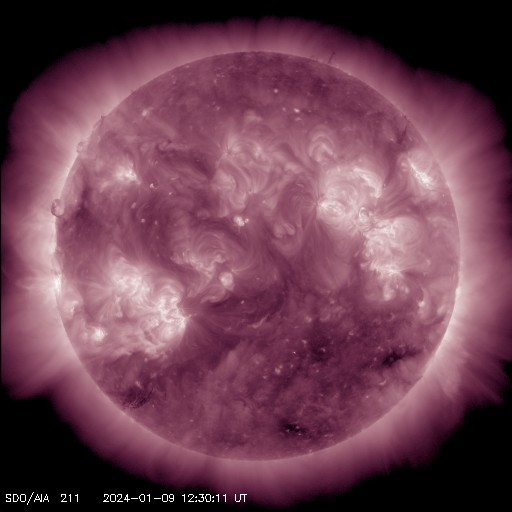
\includegraphics[width=\textwidth]{figures/latest_512_0211.jpg}
    \end{subfigure}
    \begin{subfigure}{0.5\textwidth}
      \centering
      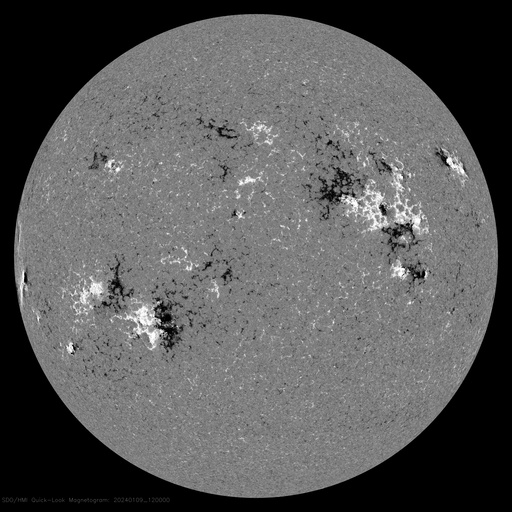
\includegraphics[width=\textwidth]{figures/latest_512_HMIB.jpg}
    \end{subfigure}
    \caption[SDO]{SDOに搭載されるAIAの211\AA フィルターによって観測される全球紫外線画像 (左)とHMIによって観測される磁場データ (右)。出典: NASA, 「SDO | Solar Dynamics Observatory」, \url{https://sdo.gsfc.nasa.gov/}(アクセス日: 2024年1月9日)}
    \label{fig:sdo_axmple}
  \end{figure}
  
  このように、現在の予測モデルにおいてはその入力データとして、観測衛星にとって得られるデータは非常に重要な役割を果たしている。

  \subsection{深層学習の活用}
    深層学習は、近年顕著な発展を遂げた機械学習の一分野である。
    効率的で高性能なモデルの登場、ハードウェアのデータ処理能力の向上、データセットの増加などがその発展を支えてきた。
    深層学習は、学術的な分野での成功のみならず、産業界においても、画像認識や自然言語処理などの分野での応用が進んでおり、情報化社会の現代においては欠かせない技術となっている。

    近年の宇宙天気予報においても、機械学習、特に深層学習アーキテクチャの基本とする予測モデルが多く開発されている (\citex{camporeale2019challenge} )。
    宇宙天気予報にとって、深層学習モデルの高速性と、不確実な現象への確率論的アプローチの有効性は特に重要な点である。
    深層学習は、蓄積された過去の大量のデータからパターンを学習するデータ駆動型のモデルであり、予測の実行は非常に高速である。
    大量の高性能なコンピューティングマシンを必要とするシミュレーションモデルより、はるかに小さい計算資源でリアルタイムでの予測が可能である。
    宇宙天気の予報は迅速に行う必要があるため、この高速性は深層学習モデルの大きな利点である。
    また、太陽フレアやコロナ質量放出などの宇宙天気現象の発生メカニズムは非常に複雑であり、完全にシミュレーションモデルで再現することは困難である。
    そのようなシステムに対して、深層学習モデルは確率論的なアプローチをとることができ、予測においてその不確実性を考慮することができる。

    宇宙天気予報における深層学習を用いた予測モデルの開発では、いくつかの注目すべき研究がある。
    \citex{nishizuka2018deep}によるDeep Flare Net (DeFN)は、太陽フレアの発生とその強度を予測するための深層学習モデルである。
    DeFNはSDOに搭載されたAIAやHMIから得られる紫外線データ、磁場データから作成された特徴量を用いて、24時間以内の太陽フレアの発生を高い精度で予測することができる。
    このモデルは予測において、注目している活動領域に対してフレアの発生とその強度を確率的に予報する。
    DeFNは、国立研究開発法人情報通信研究機構 (NICT)によって実際に運用されている。

    \citex{upendran2022global}によるDeep Lerning Geomagnetic perturbation (DAGGER)は、NASAにより開発された、衛星で観測された太陽風データをもとに、地上の地磁気摂動の予測に特化した深層学習モデルである。
    太陽フレアの爆発やCMEが発生し、地球に高エネルギー粒子が太陽風として到達すると、しばしば地磁気嵐とそれに伴う地磁気摂動が発生する。
    このような高強度の太陽風の飛来を早期に検出するために、Advanced Composition Explorer (ACE) (\citex{stone1998advanced})やWINDなどの衛星が存在する。
    これらの衛星は、地球と太陽の重力が釣り合うラグランジュ点に配置され、太陽風の強度や速度などを地球に到達する前に観測することができる。
    太陽風の速度は衛星が発する電波よりも遅く、地磁気嵐の予測においてはこの時間差をリードタイムとして利用することができる。
    しかし、高速太陽風においてはこのリードタイムは数十分程度であり、予測には高い迅速性が求められる。
    深層学習モデルであるDAGGERは、このような迅速性が求められる予測において、高い有効性を持つ。
    DAGGERが予測に要求する時間は1秒以下であり、太陽風到着までの時間的猶予がない状況でも、保護すべき技術システムに対して最大限の対応時間を与えることができる。
    
%%%%%%%%%%%%%%%%%%%%%%%%%%%%%%%%%%%%%%%%%%%%%%%%%%%%%%%%%%%%%%%%%%%%%%%%%%%%%%%%%%%%%%%%%%%%%%%%%%%%%%%%%%%%%%%%%%%%%%%%%%%%%%%%%%%%%%%%%%%%%%%%%%%%%%%%%
%%%%%%%%%%%%%%%%%%%%%%%%%%%%%%%%%%%%%%%%%%%%%%%%%%%%%%%%%%%%%%%%%%%%%%%%%%%%%%%%%%%%%%%%%%%%%%%%%%%%%%%%%%%%%%%%%%%%%%%%%%%%%%%%%%%%%%%%%%%%%%%%%%%%%%%%%

\section{問題定義}
% 「観測データ」、「深層学習の活用」、から繋げるイメージで。
% 多くのモデルや専門家による予報では、数時間後から数日後までの予報が多く、情報ソースはSDOなどの観測衛星に頼っている
% もし数日後のデータが得られれば迅速さに貢献し有用である
% 数日後のデータが得られれば有用であるが、シミュレーションモデルでの予測は計算時間などの制約で難しい、特に全球は難しい
宇宙天気予報の分野では、迅速かつ正確な予測が重要である。
現在利用されているシミュレーションモデルや深層学習モデルの多くは、数時間から数日後までの予報に焦点を当てている。
この時間範囲は、太陽の複雑でカオス的な性質を鑑みると、現在の予測モデルの現実的な限界であると考えられる。
しかし、重大な宇宙天気現象は、特に影響を受ける技術システムに対する対応策を講じる必要性があることを鑑みると、より早期に予測することが理想である。

そのために、数日後の太陽の姿を予測し、観測データとして入力とすることがアイディアとして考えられる。
それが可能であれば、既存の予測モデルのアーキテクチャを変更することなく、それらのモデルの予測可能な時間範囲をその分だけ拡張することができる。
また、専門家による主観的な予報においても、より早期に正確な予報が可能になることが期待される。
しかし、現在はそのような研究はほとんど行われておらず、その可能性は未知数である。
これにはいくつかの理由が考えられるが、太陽の時空間的特徴を正確に捉えるモデルを作成することが難しいことや、計算資源の制約などが挙げられる。
例えば、既存のMHDモデルでは、その結果として太陽の表面や大気のシミュレーションデータを得ることができるが、その計算には高い計算負荷と時間が必要であり、予測可能時間の拡大という目的で用いることは困難である。

このような問題の解決として、本研究では、深層学習による将来の太陽画像の生成という新しいアプローチを提案する。
動画予測は、深層学習の分野において近年注目されているタスクであり、その応用例は多岐にわたる。
動画予測は、動画の一部を入力として、それに続く未来の動画を予測するタスクである。
データセットとして利用できる動画や、その他の二次元の時系列データがあれば学習可能なため、動画だけではなく、気象予報や渋滞予測など、様々な分野での応用が期待されている。

本研究では、深層学習による動画予測手法を用いて、特に既存の予測モデルの入力データとして重要な、SDO / AIAから得られる全球紫外線データを予測する。
深層学習による高速な予測能力と、動画予測モデルの長期的な依存関係を学習する能力を活用し、数日後の全球紫外線画像を生成することで、より早期の宇宙天気予報の実現に貢献することを将来的な目的とする。

%%%%%%%%%%%%%%%%%%%%%%%%%%%%%%%%%%%%%%%%%%%%%%%%%%%%%%%%%%%%%%%%%%%%%%%%%%%%%%%%%%%%%%%%%%%%%%%%%%%%%%%%%%%%%%%%%%%%%%%%%%%%%%%%%%%%%%%%%%%%%%%%%%%%%%%%%
%%%%%%%%%%%%%%%%%%%%%%%%%%%%%%%%%%%%%%%%%%%%%%%%%%%%%%%%%%%%%%%%%%%%%%%%%%%%%%%%%%%%%%%%%%%%%%%%%%%%%%%%%%%%%%%%%%%%%%%%%%%%%%%%%%%%%%%%%%%%%%%%%%%%%%%%%

\section{本研究の目的}
  本研究では、深層学習による動画予測手法を用いて、SDO / AIAの時系列画像から、48時間以内の全球紫外線画像を生成することを目的とする。
  さらに、生成された画像に対して、既存の予測モデルの入力データとして用いられる輝度強度の再現性を評価することで、提案手法の有効性を検証する。
  有効性は、経度ごとでの評価や、全球のうち予測が難しいと思われる局所的な領域に対する評価、さらにシンプルなシミュレーションモデルとの比較など、さまざまな条件下で行い、モデルの時空間的ロバスト性を評価する。
  また、入力として用いる波長を変化させ、太陽表面の複雑な相互作用をモデルがどの程度モデリングできるかを評価し、その結果を考察する。

%%%%%%%%%%%%%%%%%%%%%%%%%%%%%%%%%%%%%%%%%%%%%%%%%%%%%%%%%%%%%%%%%%%%%%%%%%%%%%%%%%%%%%%%%%%%%%%%%%%%%%%%%%%%%%%%%%%%%%%%%%%%%%%%%%%%%%%%%%%%%%%%%%%%%%%%%
%%%%%%%%%%%%%%%%%%%%%%%%%%%%%%%%%%%%%%%%%%%%%%%%%%%%%%%%%%%%%%%%%%%%%%%%%%%%%%%%%%%%%%%%%%%%%%%%%%%%%%%%%%%%%%%%%%%%%%%%%%%%%%%%%%%%%%%%%%%%%%%%%%%%%%%%%

\section{本論文の構成}
  \paragraph{第2章 動画予測}
    動画予測という深層学習のタスクについて、その基本概念と基礎技術、および本研究で用いる動画予測モデルについて述べる。
  \paragraph{第3章 データ}
    本研究で用いるデータセットについて述べる。特に、各波長データの特性、およびデータセットの構築方法について述べる。
  \paragraph{第4章 Motion-Aware Unitを用いた1波長を入力とした紫外線像の全球時系列予測}
    本研究で提案する動画予測モデルを用いて、1波長を入力とした紫外線画像の全球時系列予測を行う。その結果をさまざまな条件下で評価し、モデルの有効性を検証する。
  \paragraph{第5章 Motion-Aware Unitを用いた3波長を入力とした紫外線像の全球時系列予測}
    本研究で提案する動画予測モデルを用いて、3波長を入力とした紫外線画像の全球時系列予測を行う。1波長の場合と同様に、その結果をさまざまな条件下で評価し、性能の変化とその原因を考察する。
  \paragraph{第6章 議論}
    本研究の実験全体を通した考察と、今後の展望及び課題について述べる。
  \paragraph{第7章 結論}
    本研究の結果、議論から得られた結論をまとめる。


\begin{comment}
    
そこで、まだ観測されていない未来の紫外線画像を予測、生成することで、より早期の宇宙天気予報の実現に貢献できるのではないかと考えた。

近年、深層学習技術の発展により、「動画予測(Video Prediction)」と呼ばれる技術が注目されている。動画予測とは、動画の一部を入力として、それに続く未来の動画を予測するタスクである。
動画予測を行う深層学習モデルのアーキテクチャの多くは、Long Short-Term Memory(LSTM)などの再帰的ニューラルネットワーク(RNN)のアーキテクチャを基本とする。さらに、特徴量抽出および伝播にConvolutional Neural Network(CNN)を用いることで空間的な特徴を時系列にわたってとらえ、Decoderモデルによって動画を生成する。
このような動画予測モデルは、Conv-LSTMの登場で初めて提案されて以降、様々なモデルが提案されており、自動運転や天気予報など、様々な分野での応用が期待されている。

本研究では、動画予測モデルを用いて、数日後の紫外線画像を予測、生成することを目的とする。
Deep Flare Netなどの多くの深層学習を用いた宇宙天気予報モデル、またそれらを用いた人間による主観的な宇宙天気予報は、現在の観測情報を用いて、数時間後から数日後までの宇宙天気を予測するものが多い。
それらの情報源として、数日後の高精度な紫外線画像を生成することができれば、より早期の宇宙天気予報の実現に貢献できるのではないかと考えた。

そのような数日後の紫外線像の生成のために、本研究ではMotion-Aware Unit(MAU)と呼ばれる動画予測モデルを用いる。
MAUは、RNNやCNNを用いた基本的な動画予測モデルを基本としつつ、各時間時点における画像の処理にMAU Cellと呼ばれるモジュールを多層的に積み重ねたアーキテクチャを採用している。
MAU CellはAttentionと呼ばれる機構を持ち、長期的な依存関係を適切に学習する能力を持つ。また、従来の動画予測モデルで提案されてきたEncoder-Decoderモデルや、メモリフローの改善など、様々な改良が加えられており、多くの動画予測モデルの中でも要求する計算量に対して高い予測精度を達成している。

本研究では、MAUを用いて、数日後の紫外線画像を予測、生成することを目的とするが、その評価には主に輝度強度の再現性を用いる。
これは、宇宙天気予報モデルの多くではその特徴量として輝度強度を用いていること由来する。

+シミュレーションモデルでの予測
+ 宇宙天気分野での深層学習の隆盛
+ 宇宙天気予報における紫外線画像の重要性(NICT)
+ 動画予測の応用例
+ 宇宙天気のインパクト https://link.springer.com/article/10.1186/s40623-021-01420-5
+ 過去のデータを用いたデータ駆動型のMLモデルの宇宙天気予報にける有用性

1 宇宙天気の=を予測することは大事
2 そのために観測してる
3 宇宙天気分野ではデータ駆動型の深層学習モデルが適していて、たくさん行われている
4 多くのモデルや専門家による予報では、数時間後から数日後までの予報が多く、情報ソースはSDOなどの観測衛星に頼っている
5 数日後のデータが得られれば有用であるが、シミュレーションモデルでの予測は計算時間などの制約で難しい、特に全球は
6 そこで、動画予測モデルを用いて、数日後の紫外線画像を予測、生成することを目的とする    


\end{comment}